%==============================================================================
% Figure --- T1 vs T2 at maneuver onset (case D5).  Status: READY.
% Image regenerated by scripts/analyze_onset.py from
% experiments/simulation/temporal_estimators_phase7b/onset_analysis/.
% Copied to paper/figures/fig_onset_D5.png (do not hand-edit).
%==============================================================================
\begin{figure}[t]
\centering
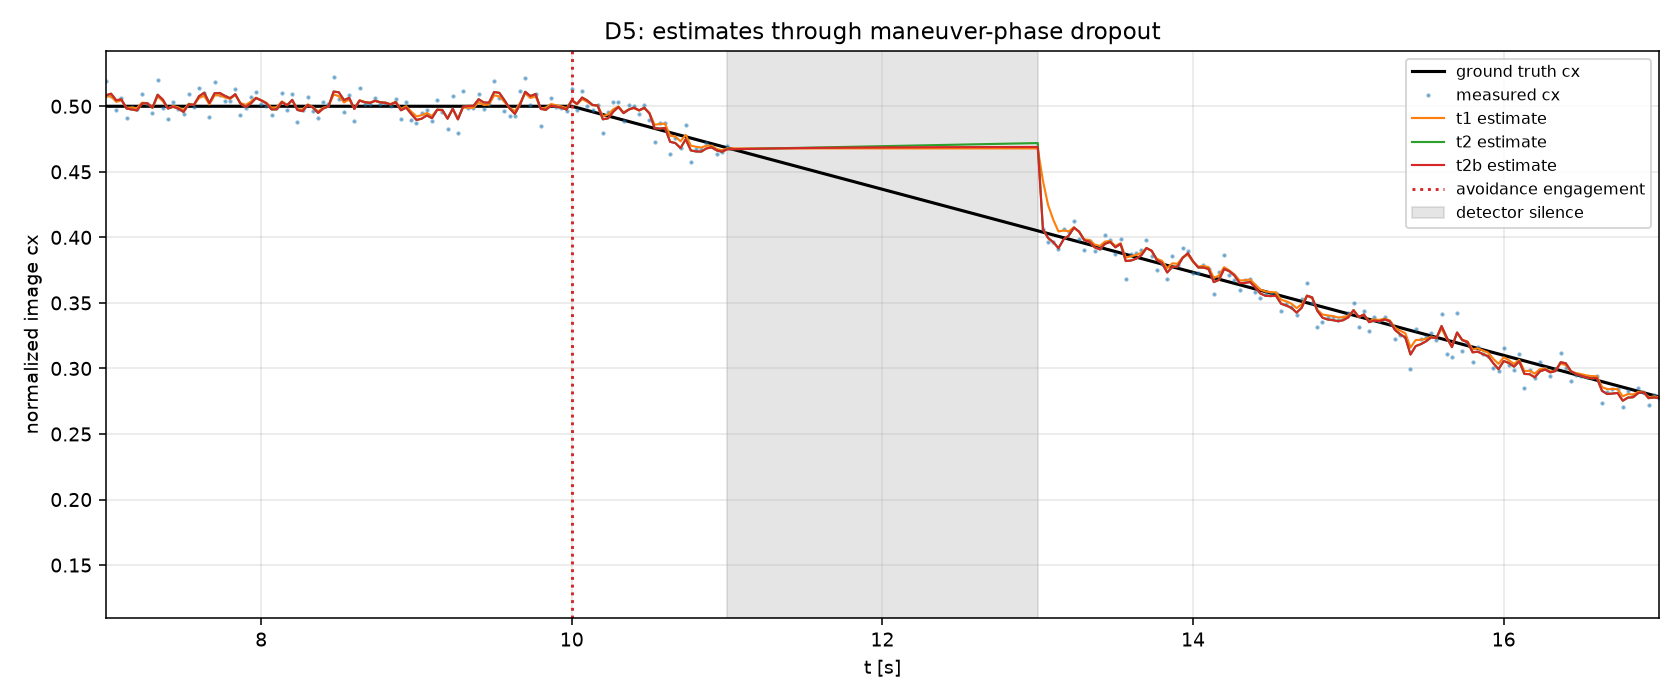
\includegraphics[width=\columnwidth]{fig_onset_D5.png}
\caption{Image-space obstacle centre during a detector dropout that begins at
maneuver onset (case D5, deterministic replay). Before commitment the
obstacle is stationary in the image; commitment introduces a step in
image-space velocity to $-0.032$\,units/s. The constant-velocity filter
extrapolates the pre-maneuver velocity through the gap and overshoots, while
the hold makes no velocity assumption. Prediction-only RMSE is 0.038 for the
hold against 0.084 for the constant-velocity filter
(Table~\ref{tab:onset}).}
\label{fig:onset}
\end{figure}
